\chapter{Toteutus}
\label{ch:toteutus}
\begin{it}
	Kirjoita tähän alkuun yleistä kamaa tästä kappaleesta mitä käsitellään ja missä järjestyksessä. Aikaisemmissa kappaleissa asetettiin jo tavoitteet ja vaatimukset ohjelmistolle. Tässä ne yhdistetään ja toteutetaan.
\end{it}


\section{Yleiskuva}
\begin{it}
	UML-kaavio kokonaisuudesta miten eri komponentit liittyvät toisiinsa ja sitä selittää auki. Mitä kirjastoa käytettiin mihinkin.
\end{it}

\begin{figure}[ht!]
	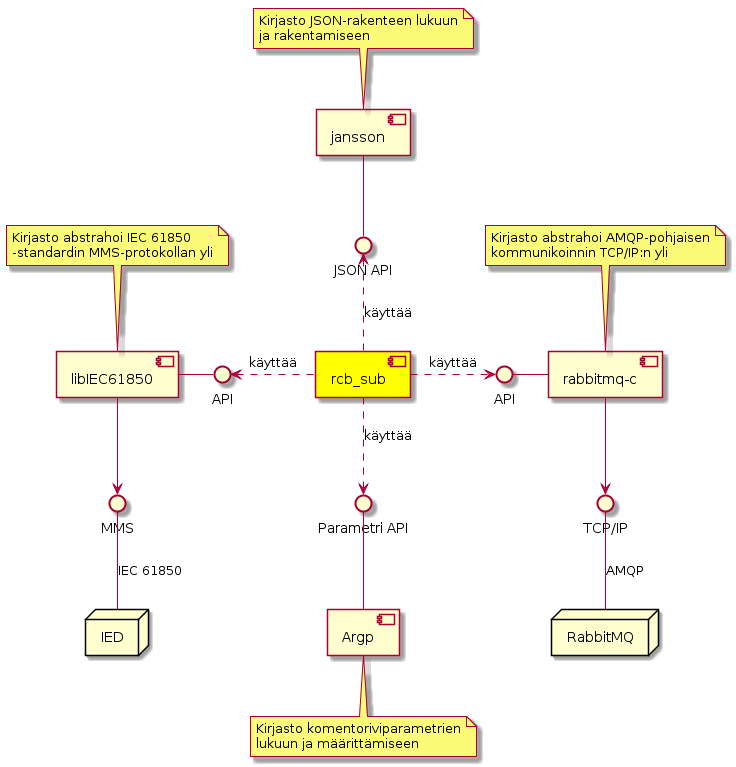
\includegraphics[width=1\textwidth]{pictures/rcb-sub-component-diagram.png}
	\caption{Toteutuksen komponenttikaavio sen osista ja relaatioista toisiinsa.}
	\label{fig:rcb-sub-komponenttikaavio}
\end{figure}



\section{Käytettyt kirjastot}
\begin{it}
	Tähän tekstiä eri kirjastoista mitä käytettiin ja mitä ne tarjosivat toteutukseen. Myös niiden APIsta voisi vähän selittää, jota sitten käytetään kun toteutusta käydään läpi.
\end{it}


\subsection{IEC 61850 -standardin ja MMS-protokollan käyttö}
\begin{it}
	IEC 61850 -standardin toteuttava C-kirjasto joka tekee raskaan työn standardin määrittämien palveluiden toteuttamiseen ja muodostamiseen. Kirjasto tarjoaa rajapinnat serveri- ja asiakasohjelmiston toteuttamiseen, mutta vain asiakasohjelmiston rajapintoja käytetään. Kirjasto tarjoaa myös rajapinnat haluttujen raporttien tilaamista varten. Kirjaston nettisivu täältä: http://libiec61850.com/libiec61850/.
\end{it}


\subsection{RabbitMQ}
\begin{it}
	RabbitMQ:n rajapinnan toteuttava kirjasto C-kielen ohjelmille. Kirjastolla voidaan toteuttaa julkaisevia ja tilaavia ohjelmistoja. Kirjastosta käytetään julkaisevan puolen toteutusta. Kirjasto löytyy täältä: https://github.com/alanxz/rabbitmq-c.
\end{it}


\subsection{JSON-formatointi}
\begin{it}
	Joku kirjasto JSON formatointiin C-kielelle. Näkyy olevan parikin vaihtoehtoa. Perustele tähän valinta ja miksi.
\end{it}


\section{Ohjelman toiminta}
\begin{it}
	UML-sekvenssikaavio ohjelman ajosta pääpiirteittäin, mitä tekee. Sitten käydä sitä läpi tekstissä ja yhdistää kirjaston rajapintoja mitä jo käsiteltiin. Yleien kuva toiminnasta ja mitä tekee missäkin järjestyksessä.
\end{it}


\section{Jatkokehitys}
\begin{it}
	Kirjoita tähän ideoita mitä jää jatkokehitykseen ja mitä ohjelmistossa on puutteita tai mitä jäi tekemättä. Esim. testaus ja CMake lisääminen.
\end{it}